\section{Related Work}
Sprachassistenten wie Amazon Alexa \cite{alexaAssitent}, Google Assistant \cite{googleAssistant}, Apple Siri \cite{siriAssistent}, Microsoft Cortana \cite{cortanaAssistent} und Baidu DuerOS \cite{baiduAssistant} dominieren aktuell den Markt und sind auf der Abbildung \ref{fig:sprachassistenten} abgebildet. Dabei gehen die Sprachassistenten unterschiedlich mit den Eingabedaten der Nutzer um. Aus den Datenschutzrichtlinien der Anbieter lassen sich meist keine exakten Information finden, was genau mit den Eingabedaten eines Nutzers passiert. Im folgenden werden die Datenschutzrichtlinien der einzelnen Anbieter kurz vorgestellt.
\begin{figure}[h!]
	\centering
	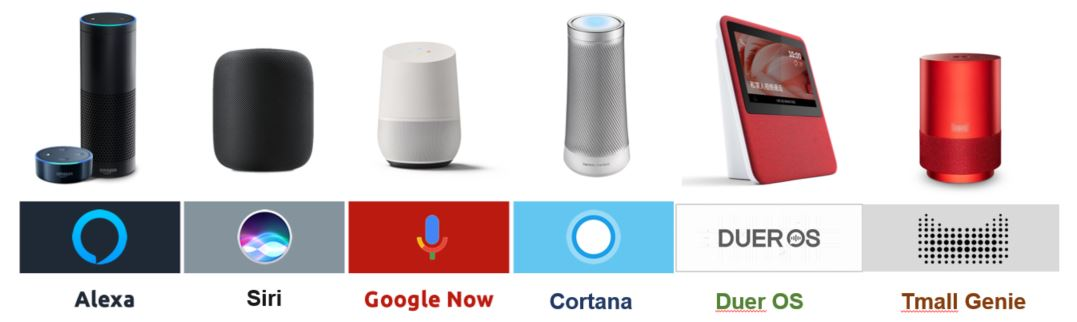
\includegraphics[width=1\linewidth]{Picture/Sprachassistenten}
	\caption[Sprachassisten auf dem MarkT]{Sprachassisten auf dem MarkT}
	\label{fig:sprachassistenten}
\end{figure}

Amazons Alexa verwendet alle Nutzereingabe, um den Sprachservice zu verbessern und personalisierte Werbung anzuzeigen. Eine Beschränkung der Datennutzung für verschiedene Bereiche ist möglich, wodurch sich allerdings auch die Funktionalität einschränkt \cite{alexaPrivacy}.

Google Assistant verwendet die gleichen Berechtigungen, welche für die mobile App des Anbieters gelten \cite{googleShare}. Eine abweichende Einstellung zur mobilen App ist dabei nicht möglich. Die Interaktion mit Google Assistant kann für die personalisiert Werbung genutzt werden, wie sonstige Suchanfragen \cite{googlePrivacy}.

Bei Siri müssen Dienste aktiviert sein, sodass darauf zugegriffen werden kann. Um die Aussprache und die Funktionalität zu verbessern werden Daten wie Name, Kontakte, Musik, Suchaktivitäten und weitere Informationen verschlüsselt übertragen. Die Daten werden nicht mit der Apple ID genutzt, sondern mit zufällig erstellten Kennung. Dadurch wird etwas Privatsphäre für Nutzer gewährleistet \cite{siriPrivacy}.

In den Datenschutzeinstellungen von Microsofts Cortana wird darüber informiert, dass bestimmte Daten \glqq [...] wie z. B. Ihre Suchen, Kalender, Kontakte und Orte. [...]\grqq{} gespeichert werden. Die Datennutzung von Cortana als Personal Assistant ist konfigurierbar. Sind die personalisierten Informationen deaktiviert, kann Cortana nur für Anwendungen wie der Suche und des Festlegung eines Timers genutzt werden. Cortana verwendet personenbezogene Daten nicht für personalisierte Werbung \cite{cortanaAssistent}. 

Baidu DuerOS sammelt ebenfalls Nutzerdaten, um die Sprachverarbeitung des Sprachassistenten zu verbessern. Qi Lu verweist auf die vielen Szenarien in denen Baidu Daten sammelt, womit Baidu den Sprung an die Weltspitze im Bereich Künstliche Intelligenz gelingen soll . Die persönlichen Daten eines Nutzers werden übermittelt. Dabei bietet Baidu keine konfigurierbare Privatsphäre an \cite{baiduAI}. 

Seit Februar gibt es den Sprachassistenten Mycroft Mark II, indem Offenheit und Privatsphäre vereint werden \cite{mycroftsmartspeaker}. Die Funktionalitäten sind hier begrenzt, da der Sprachassistent keine Daten speichert, um den Benutzerkontext weiter zu trainieren und verstehen.